\documentclass[a4paper]{article}

\usepackage[utf8]{inputenc}
\usepackage[portuges]{babel}
\usepackage{graphicx}
\usepackage{a4wide}
\usepackage[pdftex]{hyperref}
\usepackage{float}
\usepackage{indentfirst}
%\usepackage{subcaption}
\usepackage{subfig}
\usepackage{fancyhdr}

\pagestyle{fancy}
\fancyhf{}
\rhead{TP4 - Grupo 56}
\lhead{Questões e Respostas}
\rfoot{Page \thepage}

\begin{document}

\title{TP4 : Redes Sem Fios (802.11)\\ Redes e Computadores\\Grupo 56}
\author{Bruno Martins (a80410) \and Filipe Monteiro (a80229) \and Márcio Sousa (a82400)}
\date{\today}

\begin{titlepage}

  %título
  \thispagestyle{empty}
  \begin{center}
  \begin{minipage}{0.75\linewidth}
      \centering
  %engenharia logo
     
\includegraphics[width=0.4\textwidth]{pics/eng.jpeg}\par\vspace{1cm}
      \vspace{1.5cm}
  %titulos
      \href{https://www.uminho.pt/PT}{\scshape\LARGE Universidade do Minho} \par
      \vspace{1cm}
      \href{https://www.di.uminho.pt/}{\scshape\Large Departamento de Informática} \par
      \vspace{1.5cm}

  \maketitle
  \end{minipage}
  \end{center}

  \vspace{2cm}

  


  \clearpage

 \end{titlepage}
 \tableofcontents
 \newpage
 
 \section{Acesso Rádio}
 \subsection{Identifique em que frequência do espectro está a operar a rede sem fios, e o
canal que corresponde essa frequência.}
Analisando a trama 356 (grupo 56), verificamos que a frequência em que está a operar a rede sem fios é de 2467MHz, no canal 12.
\begin{figure}[H]
\centering
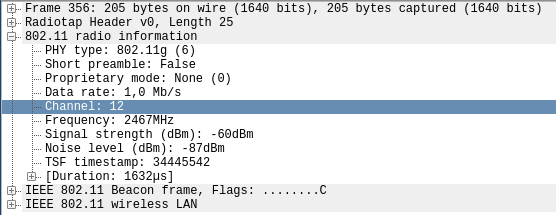
\includegraphics[scale=0.50]{pics/p1.png}
\caption{Informação do cabeçalho do do nível físico \textit{radio information}}
\end{figure}

 \subsection{Identifique a versão da norma IEEE 802.11 que está a ser usada.}
\begin{figure}[H]
\centering
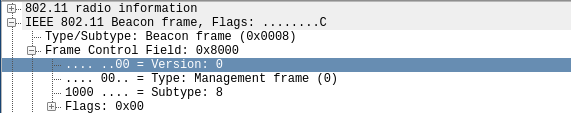
\includegraphics[scale=0.60]{pics/p2.png}
\caption{Versão da norma IEEE 802.11}
\end{figure}
Está a ser usada a versão 0 da norma IEEE 802.11 (\textit{standard}).

 \subsection{Qual o débito a que foi enviada a trama escolhida? Será que esse débito
corresponde ao débito máximo a que a interface WiFi pode operar? Justifique.}
\begin{figure}[H]
\centering
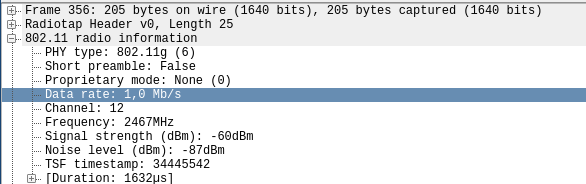
\includegraphics[scale=0.50]{pics/p3-1.png}
\caption{Débito a que foi transmitido a trama}
\end{figure}

\begin{figure}[H]
\centering
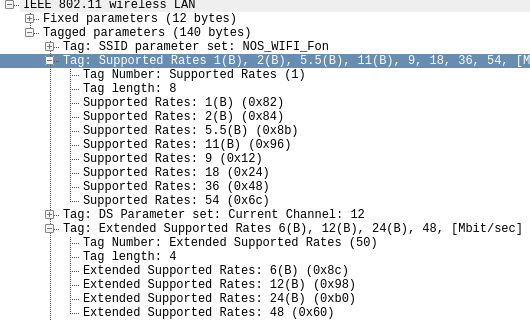
\includegraphics[scale=0.50]{pics/p3-2.png}
\caption{Vários débitos suportados pela interface}
\end{figure}
Foi enviada a um débito de 1Mb/s mas a place de rede suportava débitos maiores pois no campo \textit{supported rates} existem outros débitos maiores que o usado.
 

\section{Scanning Passivo e Scanning Ativo}
\setcounter{subsection}{3}

\subsection{Selecione uma trama beacon (e.g., a trama 3XX). Esta trama pertence a que tipo
de tramas 802.11? Indique o valor dos seus identificadores de tipo e de subtipo.
Em que parte concreta do cabeçalho da trama estão especificados (ver anexo)?}

Esta trama pertence ao tipo \textit{Management Frame} (0) e ao subtipo \textit{Beacon} (8). 
\begin{figure}[H]
\centering
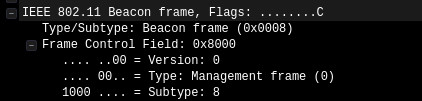
\includegraphics[scale=0.50]{pics/p4.png}
\caption{Parte do cabeçalho da trama Beacon}
\end{figure}


\subsection{Liste todos os SSIDs dos APs (Access Points) que estão a operar na vizinhança da
STA de captura? Explicite o modo como obteve essa informação. Como sugestão
pode construir um filtro de visualização apropriado (tomando como base a
resposta da alínea anterior) que lhe permita obter a listagem pretendida.}
Os SSIDs são \textit{NOS\_WIFI\_Fon} e \textit{FlyingNet}.
Para facilitar a procura dos SSIDs, aplicamos o filtro \textbf{wlan.fc.type\_subtype == 0x0008} para filtrar apenas os \textit{Beacon} e depois tornamos o campo SSID do cabeçalho do IEEE802.11 numa coluna, ordenando por esta.
\begin{figure}[H]
\centering
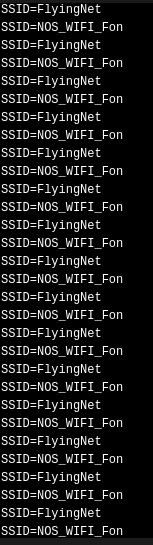
\includegraphics[scale=0.50]{pics/p5.png}
\caption{SSIDs dos ARPs da captura}
\end{figure}

\subsection{Verifique se está a ser usado o método de detecção de erros (CRC), e se todas as
tramas Beacon são recebidas corretamente. Justifique o porquê de usar detecção
de erros neste tipo de redes locais.}
Está a ser usado CRC porque a trama está a utilizar Frame Check Sequence, que é um algoritmo de Cycle Redundancy Check. Todas as tramas são recebidas corretamente pois quando se aplica o filtro no wireshark para apenas mostrar as tramas com FCS incorreto nao é mostrada nenhuma.
\begin{figure}[H]
\centering
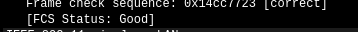
\includegraphics[scale=0.70]{pics/p6.png}
\caption{Utilização de FCS}
\end{figure}

\subsection{Para dois dos APs identificados, indique qual é o intervalo de tempo previsto
entre tramas beacon consecutivas?	 	 (Nota: este valor é anunciado na própria
trama beacon). Na prática, a periodicidade de tramas beacon é verificada? Tente
explicar porquê.}
O intervalo de tempo entre as tramas é de 100ms. Verifica-se que numa das redes existentes (\textit{NOS\_WIFI\_ZON}) não respeitava a periocidade anunciada (valores mais baixos que o esperado).
\begin{figure}[H]
\centering
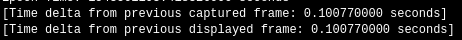
\includegraphics[scale=0.50]{pics/p7.png}
\caption{ntervalo de tempo das tramas Beacon}
\end{figure}

\subsection{Identifique e registe todos os endereços MAC usados nas tramas beacon
enviadas pelos APs. Recorde que o endereçamento está definido no cabeçalho
das tramas 802.11, podendo ser utilizados até quatro endereços com diferente
semântica.	 	 Para uma descrição detalhada da estrutura da trama 802.11,
consulte o anexo ao enunciado.}

\begin{figure}[H]
\centering
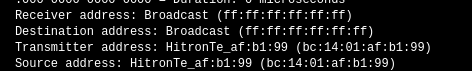
\includegraphics[scale=0.50]{pics/p8.png}
\caption{Endereços Mac das tramas Beacon}
\end{figure}



\subsection{As tramas beacon anunciam que o AP pode suportar vários débitos de base
assim como vários “extended supported rates”.		Indique quais são esses débitos?}
Os débitos dos APs podem ser verificados nas imagens seguintes:
\begin{figure}[H]
\centering

\includegraphics[scale=0.60]{pics/p91.png}
\caption{Débito base}
\end{figure}
\begin{figure}[H]
\centering

\includegraphics[scale=0.60]{pics/p9.png}
\caption{Débito do "extended supported rates"}
\end{figure}


\subsection{Estabeleça um filtro Wireshark apropriado que lhe permita visualizar todas as
tramas probing request ou probing response, simultaneamente.}
\begin{figure}[H]
\centering
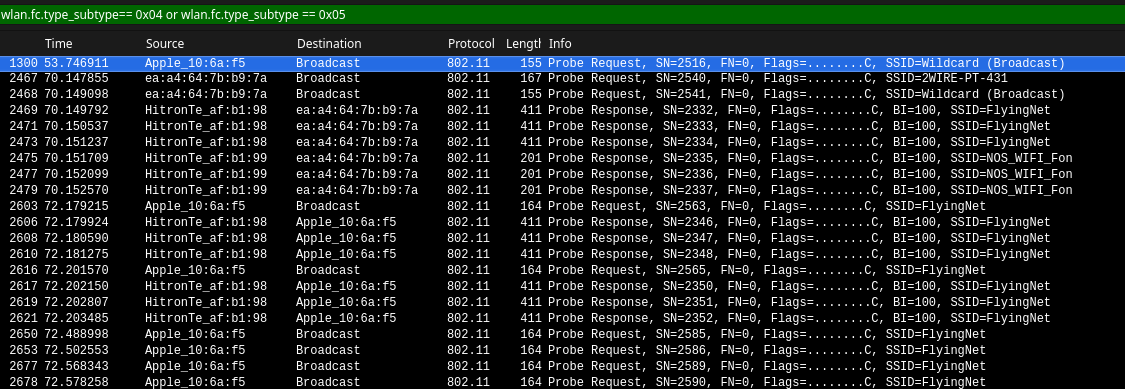
\includegraphics[scale=0.30]{pics/p10.png}
\caption{Tramas de request  com o filtro na parte verde}
\end{figure}
\subsection{Identifique um probing request para o qual tenha havido um probing response.}
Na primeira imagem a trama selecionada é um request, e na segunda a trama selecionada é a resposta ao request.
\begin{figure}[H]
\centering
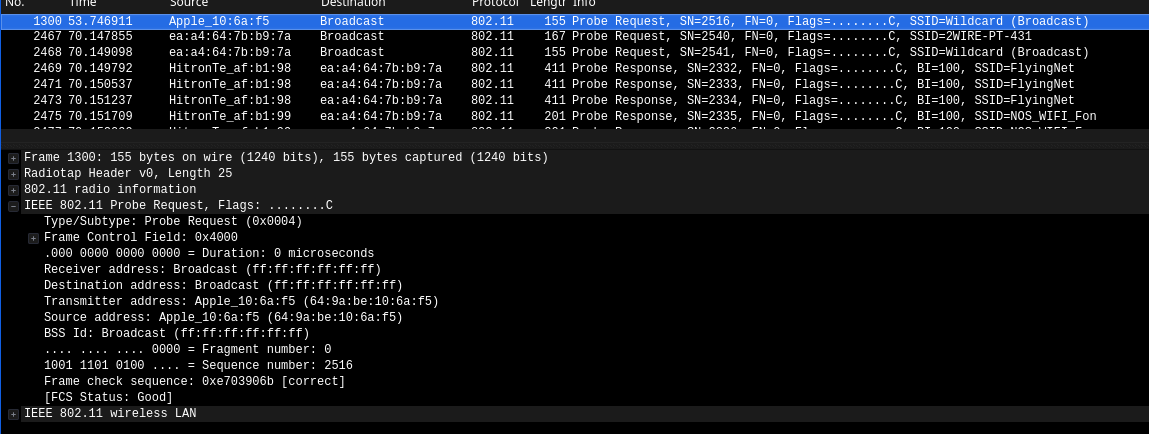
\includegraphics[scale=0.30]{pics/p111.png}
\caption{Probe Request}
\end{figure}
\begin{figure}[H]
\centering
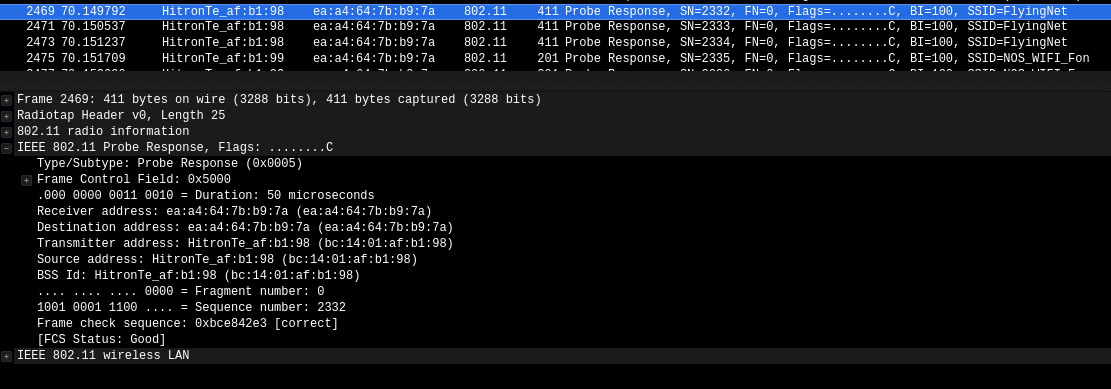
\includegraphics[scale=0.30]{pics/p112.png}
\caption{Probe response}
\end{figure}



\section{Processo de Associação}
\setcounter{subsection}{11}

\subsection{Identifique uma sequência de tramas que corresponda a um processo de
associação completo entre a STA e o AP, incluindo a fase de autenticação.}
\begin{figure}[H]
\centering
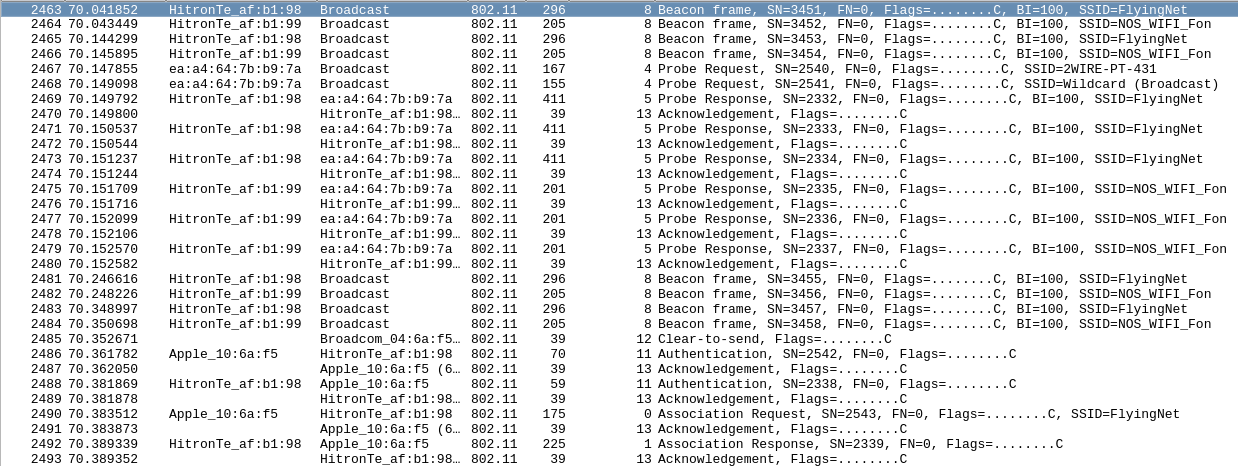
\includegraphics[scale=0.30]{pics/p12.png}
\caption{Sequencia de frames de um processo de associação completo entre uma\textit{Station} e uma \textit{AP}}
\end{figure}
Da frame 2464 até á 2493 foi associado o dispositivo com MAC \textit{Apple\_10:6a:f5.} ao AP com MAC  \textit{bc:14:01:af:b1:98}.


\subsection{Efetue um diagrama que ilustre a sequência de todas as tramas trocadas no
processo}
\begin{figure}[H]
\centering
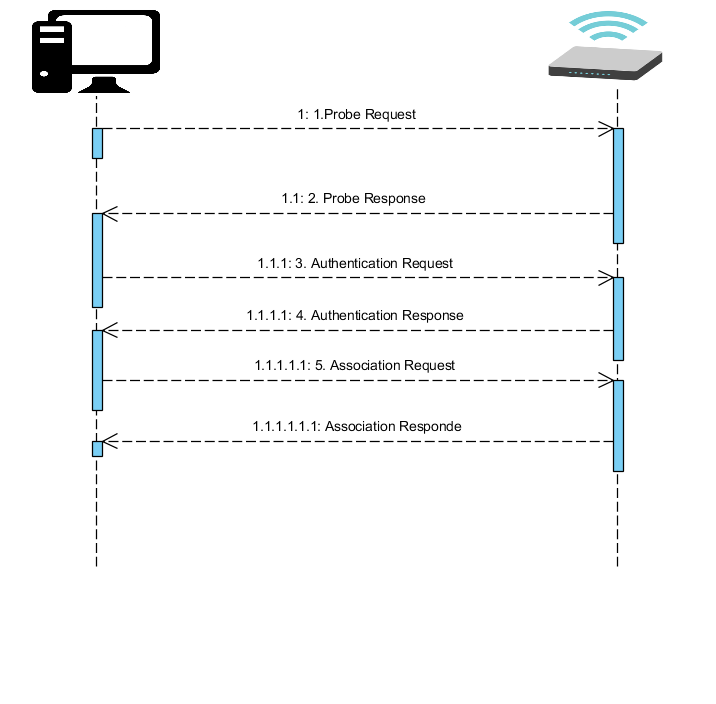
\includegraphics[scale=0.50]{pics/diagrama.png}
\caption{Diagrama com o processo de associação}
\end{figure}



\section{Transferência de Dados}
\setcounter{subsection}{13}

\subsection{Considere a trama de dados nº455. Sabendo que o campo Frame Control contido
no cabeçalho das tramas 802.11 permite especificar a direccionalidade das
tramas, o que pode concluir face à direccionalidade dessa trama, será local à
WLAN?}
Pode concluir-se que não é local á WLAN, pois a trama vem de um sistema de distribuição (DS) para o dispositivo \textit{host}, através do ponto de acesso (visível na \textit{Flag} "DS status").
\begin{figure}[H]
\centering
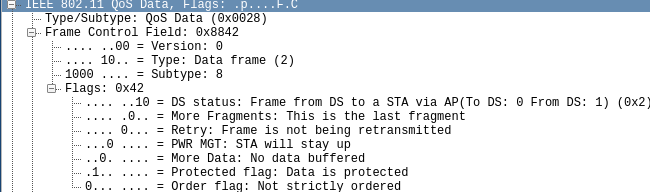
\includegraphics[scale=0.50]{pics/p14.png}
\caption{Campo Frame Control da trama}
\end{figure}



\subsection{Para a trama de dados nº455, transcreva os endereços MAC em uso,
identificando qual o endereço MAC correspondente ao host sem fios (STA), ao AP
e ao router de acesso ao sistema de distribuição?}
\begin{figure}[H]
\centering
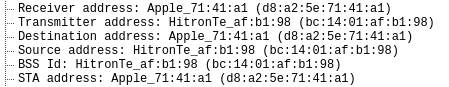
\includegraphics[scale=0.70]{pics/p15.png}
\caption{Vários campos com os vários endereços MAC}
\end{figure}
\begin{itemize}
    \item MAC STA: d8:a2:5e:71:41:a1
    \item MAC AP: bc:14:01:af:b1:98	
    \item MAC Router: bc:14:01:af:b1:98
\end{itemize}
Neste caso, o router para além de AP, é o ponto de ligação com o sistema de distribuição.

\subsection{Como interpreta a trama nº457 face à sua direccionalidade e endereçamento
MAC?}
Esta trama está a ser enviada do dispositivo \textit{host} (STA) para o sistema de distribuição através (DS) através do ponto de acesso (AP).

\subsection{Que subtipo de tramas de controlo são transmitidas ao longo da transferência de
dados acima mencionada? Tente explicar porque razão têm de existir
(contrariamente ao que acontece numa rede Ethernet.)}
Os subtipos existentes nas tramas de controlo ao longo da transferência de dados são os seguintes:
\begin{itemize}
    \item 8 - \textit{Block Ack Request}
    \item 9 - \textit{Block Ack}
    \item 11 - \textit{RTS}
    \item 12 - \textit{CTS}
    \item 13 - \textit{ACK}
\end{itemize}
Existem porque apenas um dispositivo pode comunicar de cada vez com o AP, sendo necessário o controlo de quem está a comunicar e quando termina para outro poder começar. Numa rede Ethernet isto não é necessário pois cada dispositivo tem um dominio de colisão diferente (em IEEE802.11 o espaço é partilhado podendo haver colisão).


\subsection{O uso de tramas Request To Send e Clear To Send, apesar de opcional, é comum
para efetuar "pré-reserva" do acesso ao meio quando se pretende enviar tramas
de dados, com o intuito de reduzir o número de colisões resultante
maioritariamente de STAs escondidas. Para o exemplo acima, verifique se está a
ser usada a opção RTS/CTS na troca de dados entre a STA e o AP/Router da
WLAN, identificando a direccionalidade das tramas e os sistemas envolvidos.}
\begin{figure}[H]
\centering
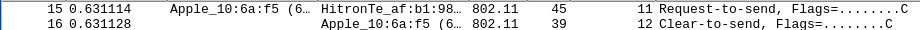
\includegraphics[scale=0.5]{pics/p18.png}
\caption{Exemplo de duas tramas - uma RTS e outra CTS - usadas na troca de dados entre STA e AP/Router}
\end{figure}
Verifica-se que está a ser usado RTS e CTS sendo que nas tramas apresentadas na figura, a primeira é \textit{Station} 64:9a:be:10:6a:f5 a enviar um RTS e na seguinte o AP/ROuter bc:14:01:af:b1:98 envia um CTS, concedendo permissão a transferir dados.



\section{Conclusão}
Este trabalho incidiu no que diz respeito ao protocolo IEEE 802.11, tanto a nível do formato
das suas tramas, como ao nível do endereçamento dos componentes que constituem a comunicação sem fios. 
Relativamente a tramas, sabemos agora que estas se dividem em três tipos, Tramas de Gestão que, tal como o seu nome diz, são as responsáveis pela gestão da comunicação entre os vários participantes da rede (\textit{stations, AP and routers}, isto é, pelo estabelecimento e manutenção da comunicação, Tramas de Controlo que controlam o envio e receção de mensagens, e Tramas de Dados, responsáveis pela transmissão de dados.
Foi abordado também como os nossos dispositivos conseguem encontrar, aceder e usar uma rede sem fios.
\end{document}
